\pdfobjcompresslevel 0
\documentclass[
11pt, % The default document font size, options: 10pt, 11pt, 12pt
%oneside, % Two side (alternating margins) for binding by default, uncomment to switch to one side
%chapterinoneline,% Have the chapter title next to the number in one single line
french, % ngerman for German
singlespacing, % Single line spacing, alternatives: onehalfspacing or doublespacing
%draft, % Uncomment to enable draft mode (no pictures, no links, overfull hboxes indicated)
%nolistspacing, % If the document is onehalfspacing or doublespacing, uncomment this to set spacing in lists to single
%liststotoc, % Uncomment to add the list of figures/tables/etc to the table of contents
%toctotoc, % Uncomment to add the main table of contents to the table of contents
%parskip, % Uncomment to add space between paragraphs
%nohyperref, % Uncomment to not load the hyperref package
headsepline, % Uncomment to get a line under the header
]{MastersDoctoralThesis} % The class file specifying the document structure

\usepackage[utf8]{inputenc}
\DeclareUnicodeCharacter{2010}{-}
%\usepackage[french]{babel}
\usepackage{amsmath}
\usepackage{lmodern}
\usepackage{amsfonts}
\usepackage{amssymb}
\usepackage{graphicx}
\usepackage{color}
\usepackage{xcolor}
\usepackage{url}
\usepackage{subcaption}
\usepackage{glossaries}
\usepackage{hyperref}
\usepackage{palatino} % Use the Palatino font by default
\usepackage{minitoc}


%\usepackage[backend=bibtex,style=authoryear,natbib=true]{biblatex} % Use the bibtex backend with the authoryear citation style (which resembles APA)
 
%\addbibresource{biblio.bib} % The filename of the bibliography
 
\usepackage[autostyle=true]{csquotes} % Required to generate language-dependent quotes in the bibliography

%-------------------------------
% COLOR SETTINGS


\definecolor{olivegreen}{RGB}{207,228,50}
\definecolor{briquered}{RGB}{155,61,34}
\definecolor{semilightblue}{RGB}{52,153,255}
\definecolor{pinkyred}{RGB}{255,103,103}

\definecolor{plum}{HTML}{92268F}
\definecolor{oliveGreen}{HTML}{007E00}

\definecolor{rose_cochon}{HTML}{CE6363}
\definecolor{bleu_random}{HTML}{002CA6}
\definecolor{violet_cool}{HTML}{4E005C}
\definecolor{vert_fonce}{HTML}{005413}

\definecolor{brique}{HTML}{B9655E}
\definecolor{vert_turquoise}{HTML}{53C36A}
\definecolor{bleu_window}{HTML}{3E9BDA}


\definecolor{bleu_transparent}{HTML}{0088B1}
%-------------------------------


 
\usepackage[textsize=footnotesize,obeyFinal]{todonotes}
\setlength{\marginparwidth}{2.5cm}
\newcommand{\note}[1]{\todo[color=orange!80]{#1}\ }
\newcommand{\inline}[1]{\todo[color=orange!80, inline]{#1}}

\newcommand{\resume}[1]{
	\begin{colbox}{D0D0D0}
	\textbf{Résumé}
	
	#1
	\end{colbox}
}
	
\newsavebox{\selvestebox}
\newenvironment{colbox}[1]
  {\newcommand\colboxcolor{#1}%
   \begin{lrbox}{\selvestebox}%
   \begin{minipage}{\dimexpr\columnwidth-2\fboxsep\relax}}
  {\end{minipage}\end{lrbox}%
   \begin{center}
   \colorbox[HTML]{\colboxcolor}{\usebox{\selvestebox}}
   \end{center}}


\DeclareMathOperator*{\argmin}{arg\,min}

\newcommand{\groupcharac}[3]{
\begin{figure}[h]
	\centering
	\begin{subfigure}{0.4\linewidth}
		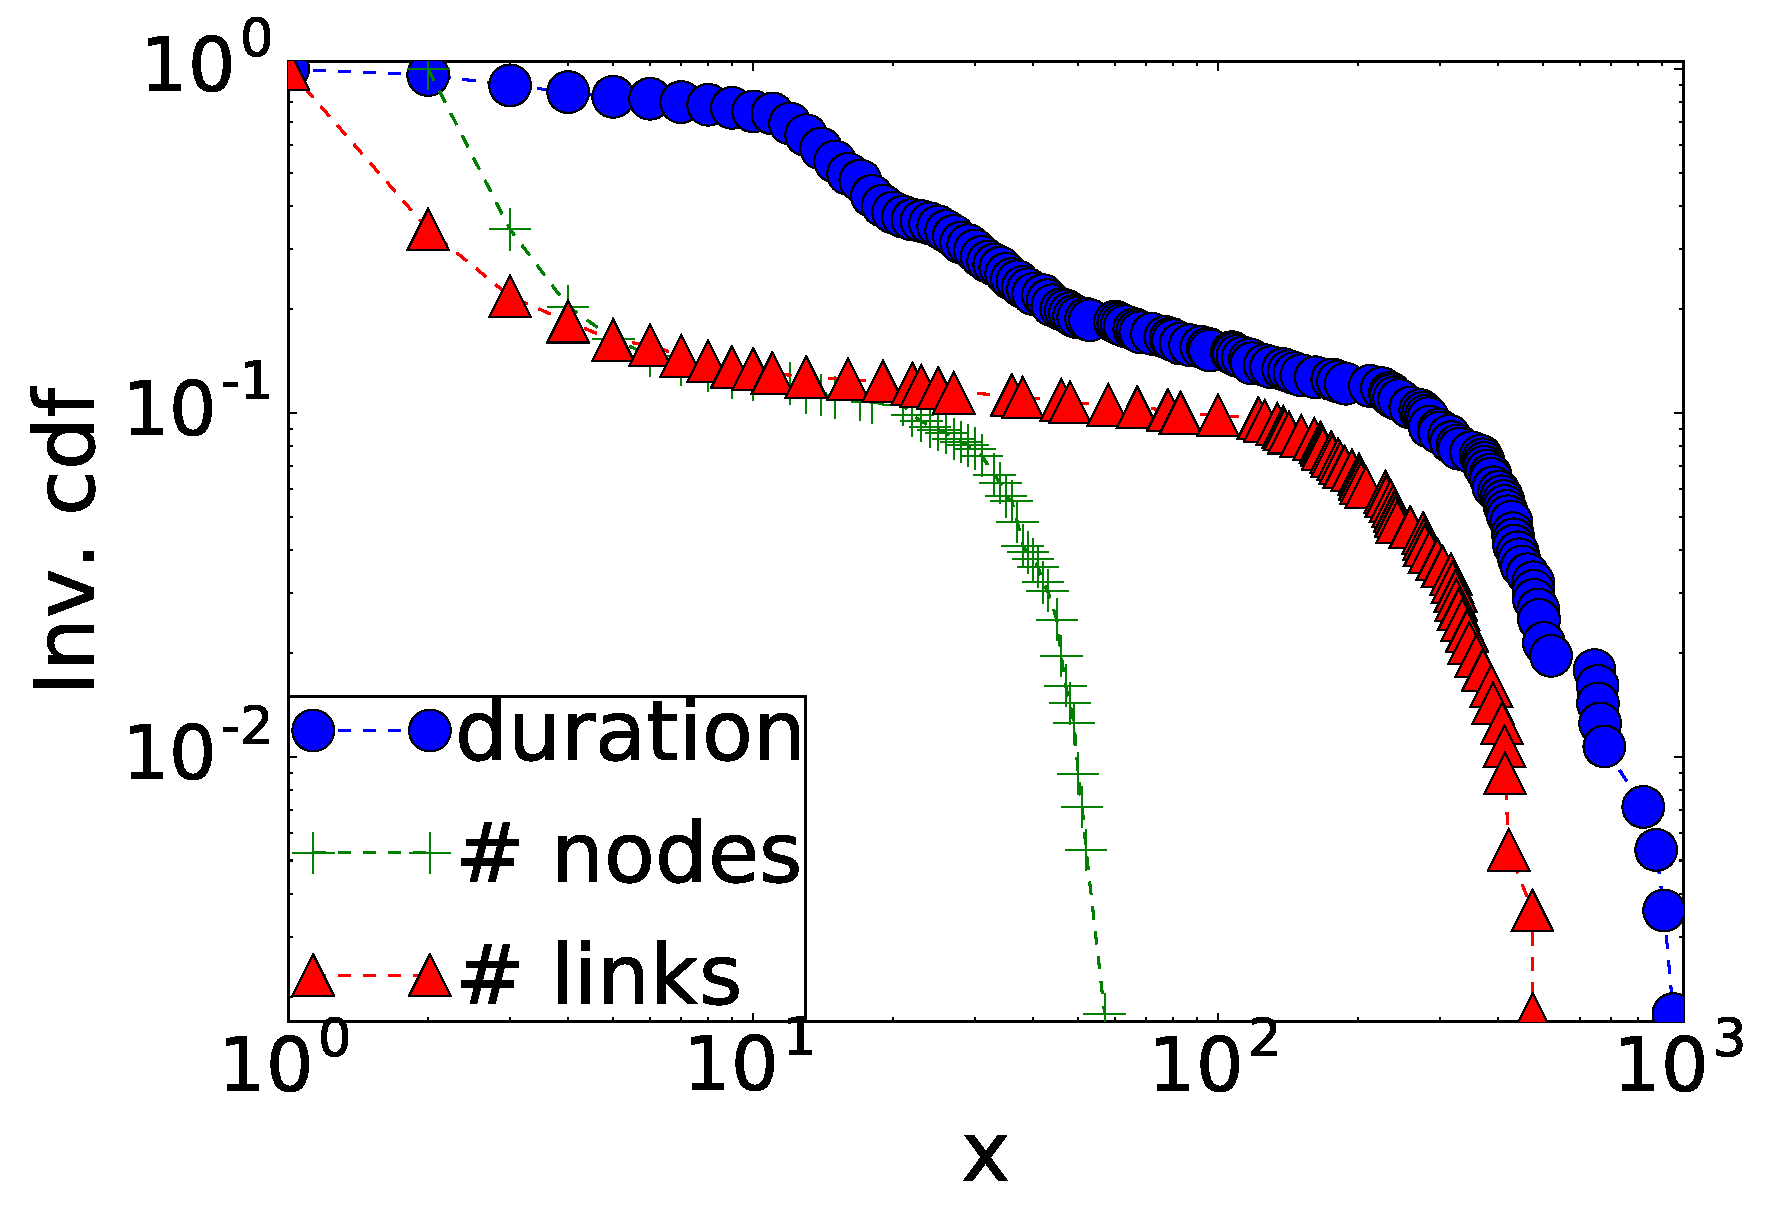
\includegraphics[width=\linewidth]{img/GroupeDense/#1/filter/Distrib_avant_filtre_best}
	\end{subfigure}\hspace{0.03\linewidth}
	\begin{subfigure}{0.4\linewidth}
		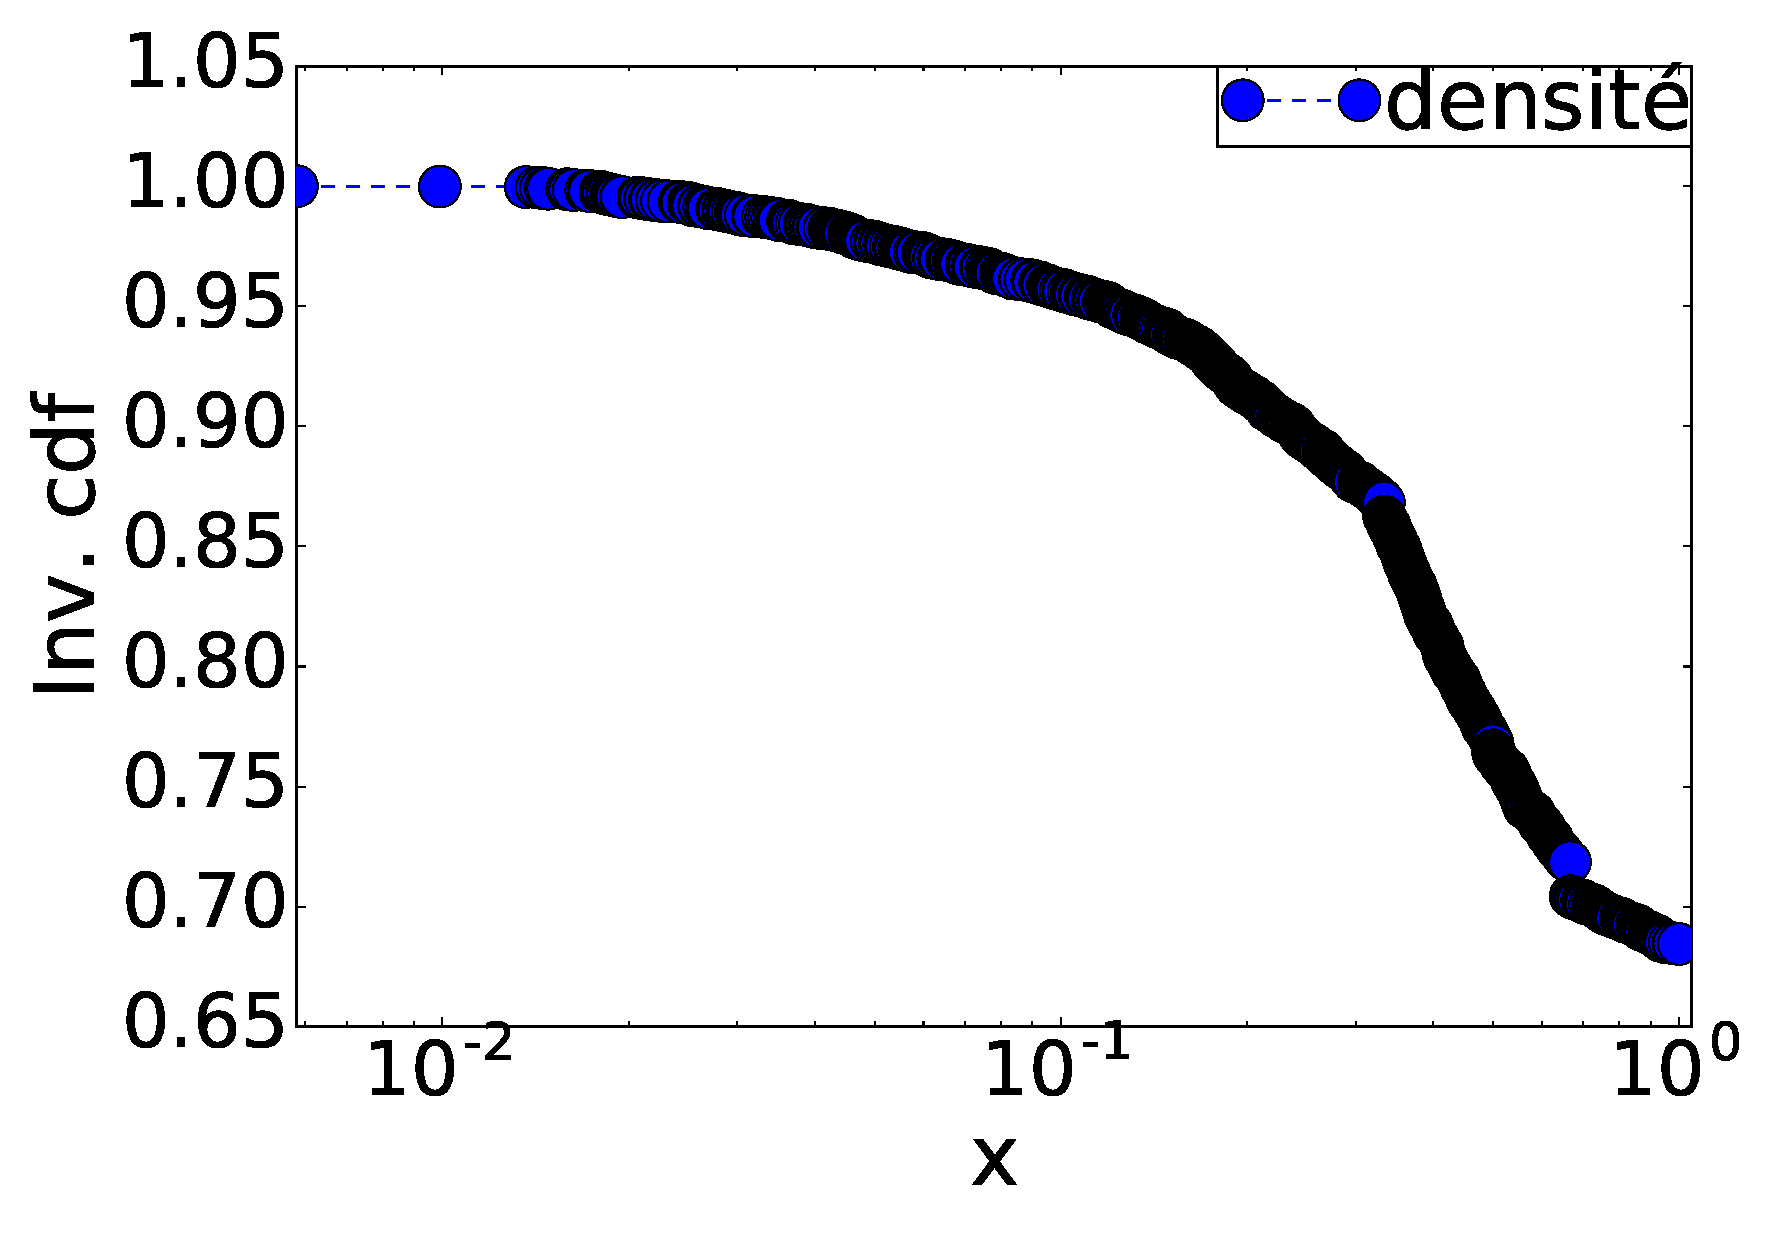
\includegraphics[width=\linewidth]{img/GroupeDense/#1/filter/Distrib_avant_dens.eps}
	\end{subfigure}
	\caption{Inverse cumulative distributions of the number of links, nodes and duration in (a) and density in (b) for the candidates found by the Louvain method on the #2 dataset.}
	\label{fig:distri_group_#3}
\end{figure}
}

\newcommand{\groupsPerNode}[3]{
	\begin{figure}[h]
	\centering
	
	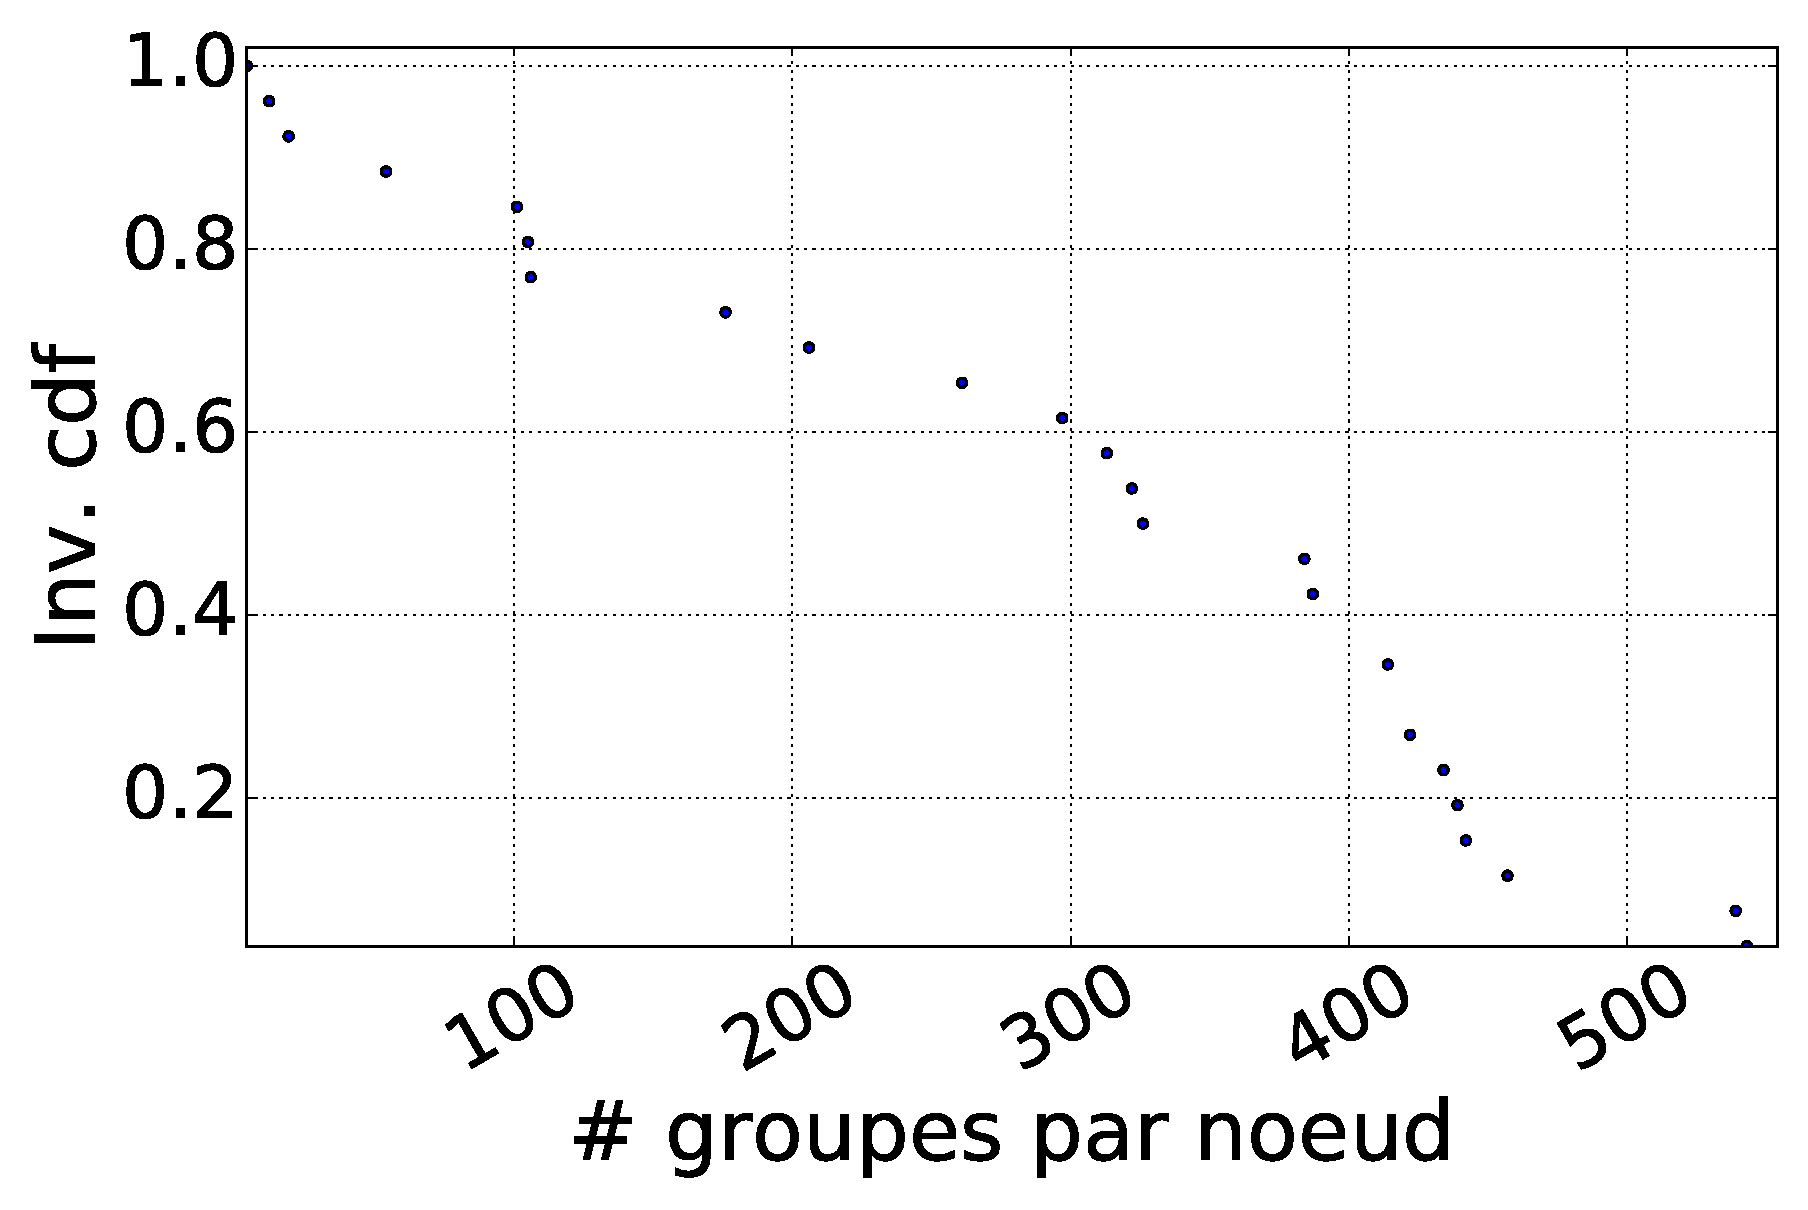
\includegraphics[width=0.5\linewidth]{img/GroupeDense/#1/filter/Prop_node.eps}
	\caption{Inverse cumulative distribution of the number of groups captured per node for the #2 dataset.}
	\label{fig:ditribnodes_#3}
	\end{figure}
}

\newcommand{\percentile}[3]{
	\begin{figure}[h]
	\centering
	
	\begin{subfigure}{0.48\linewidth}
		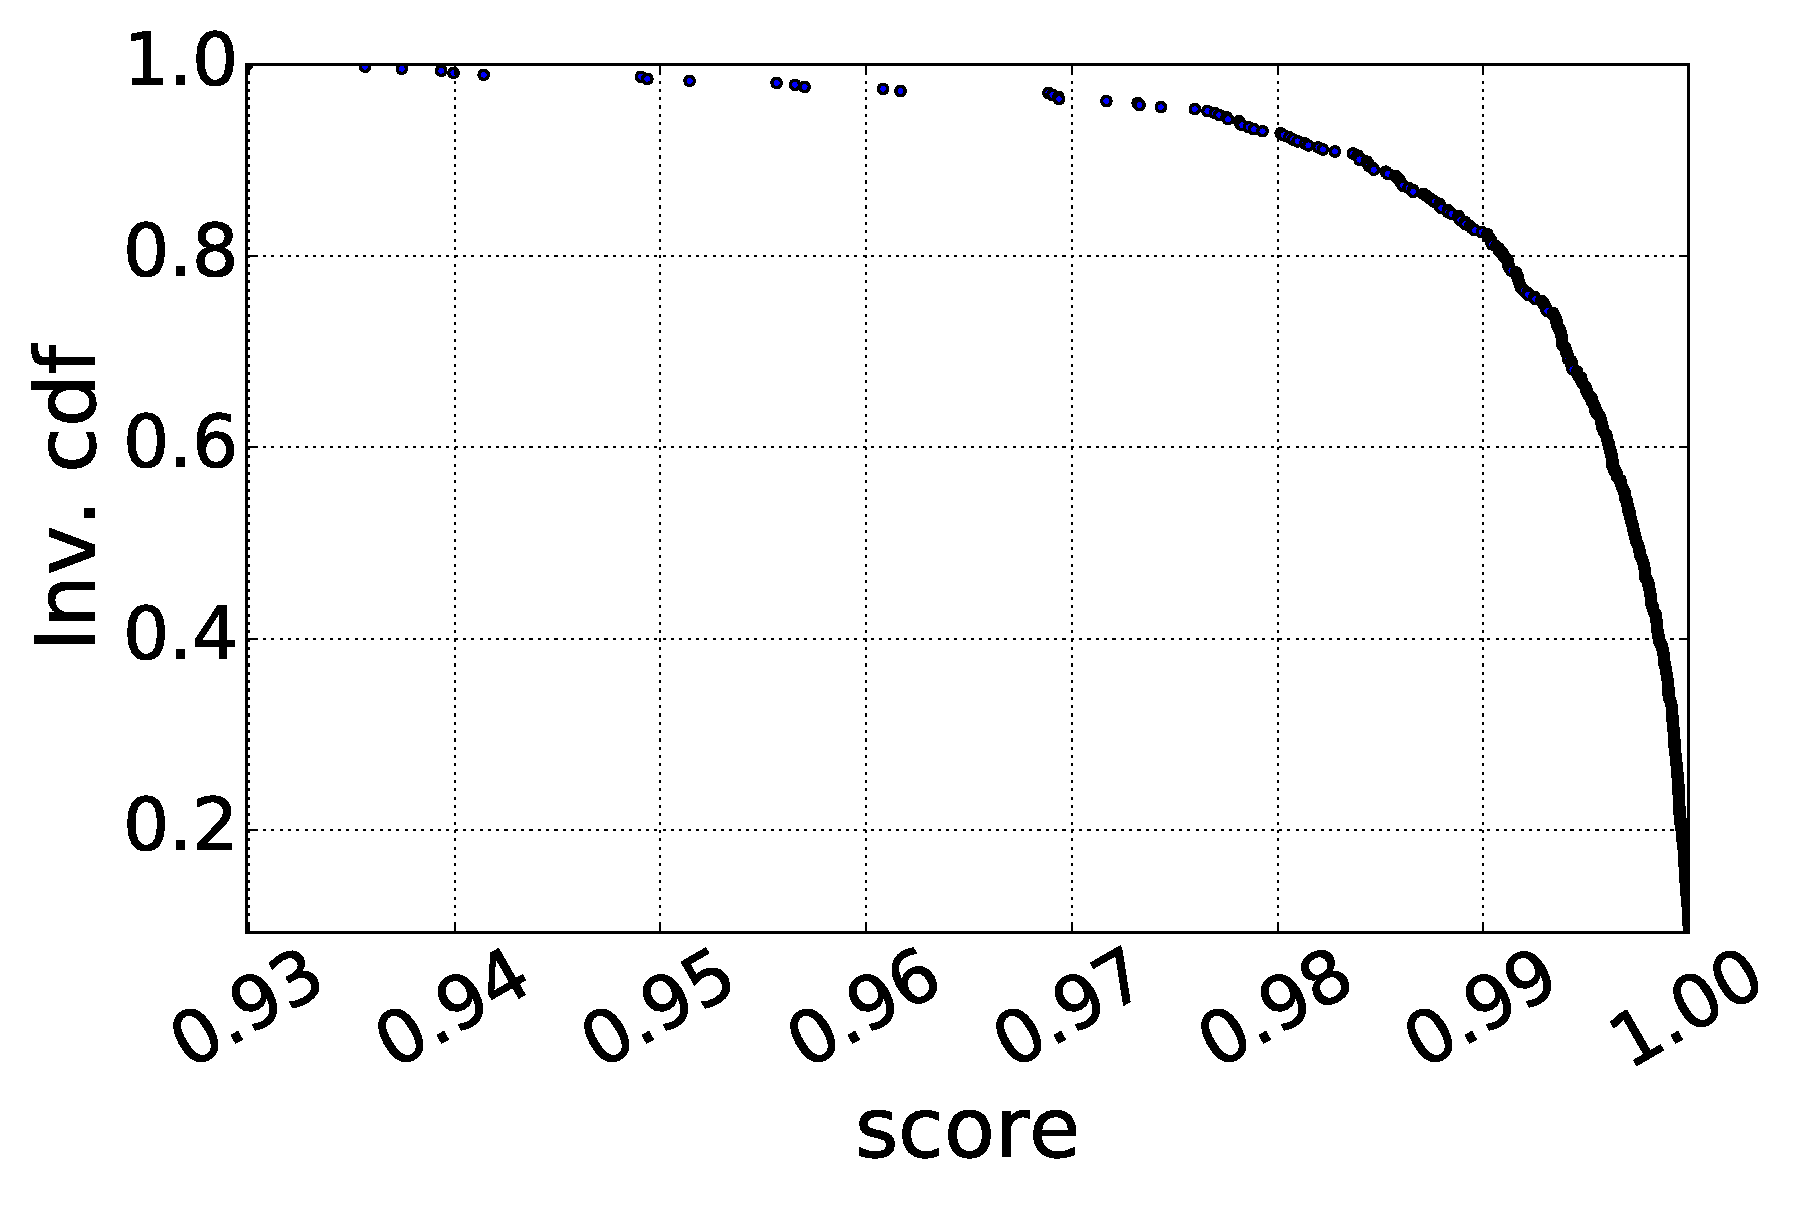
\includegraphics[width=\linewidth]{img/GroupeDense/#1/Percentil/Distribution_percentil_FixDuration_top155.eps}
		\caption{Start time: $p_{t}$}
	\end{subfigure}\hfill
	\begin{subfigure}{0.48\linewidth}
		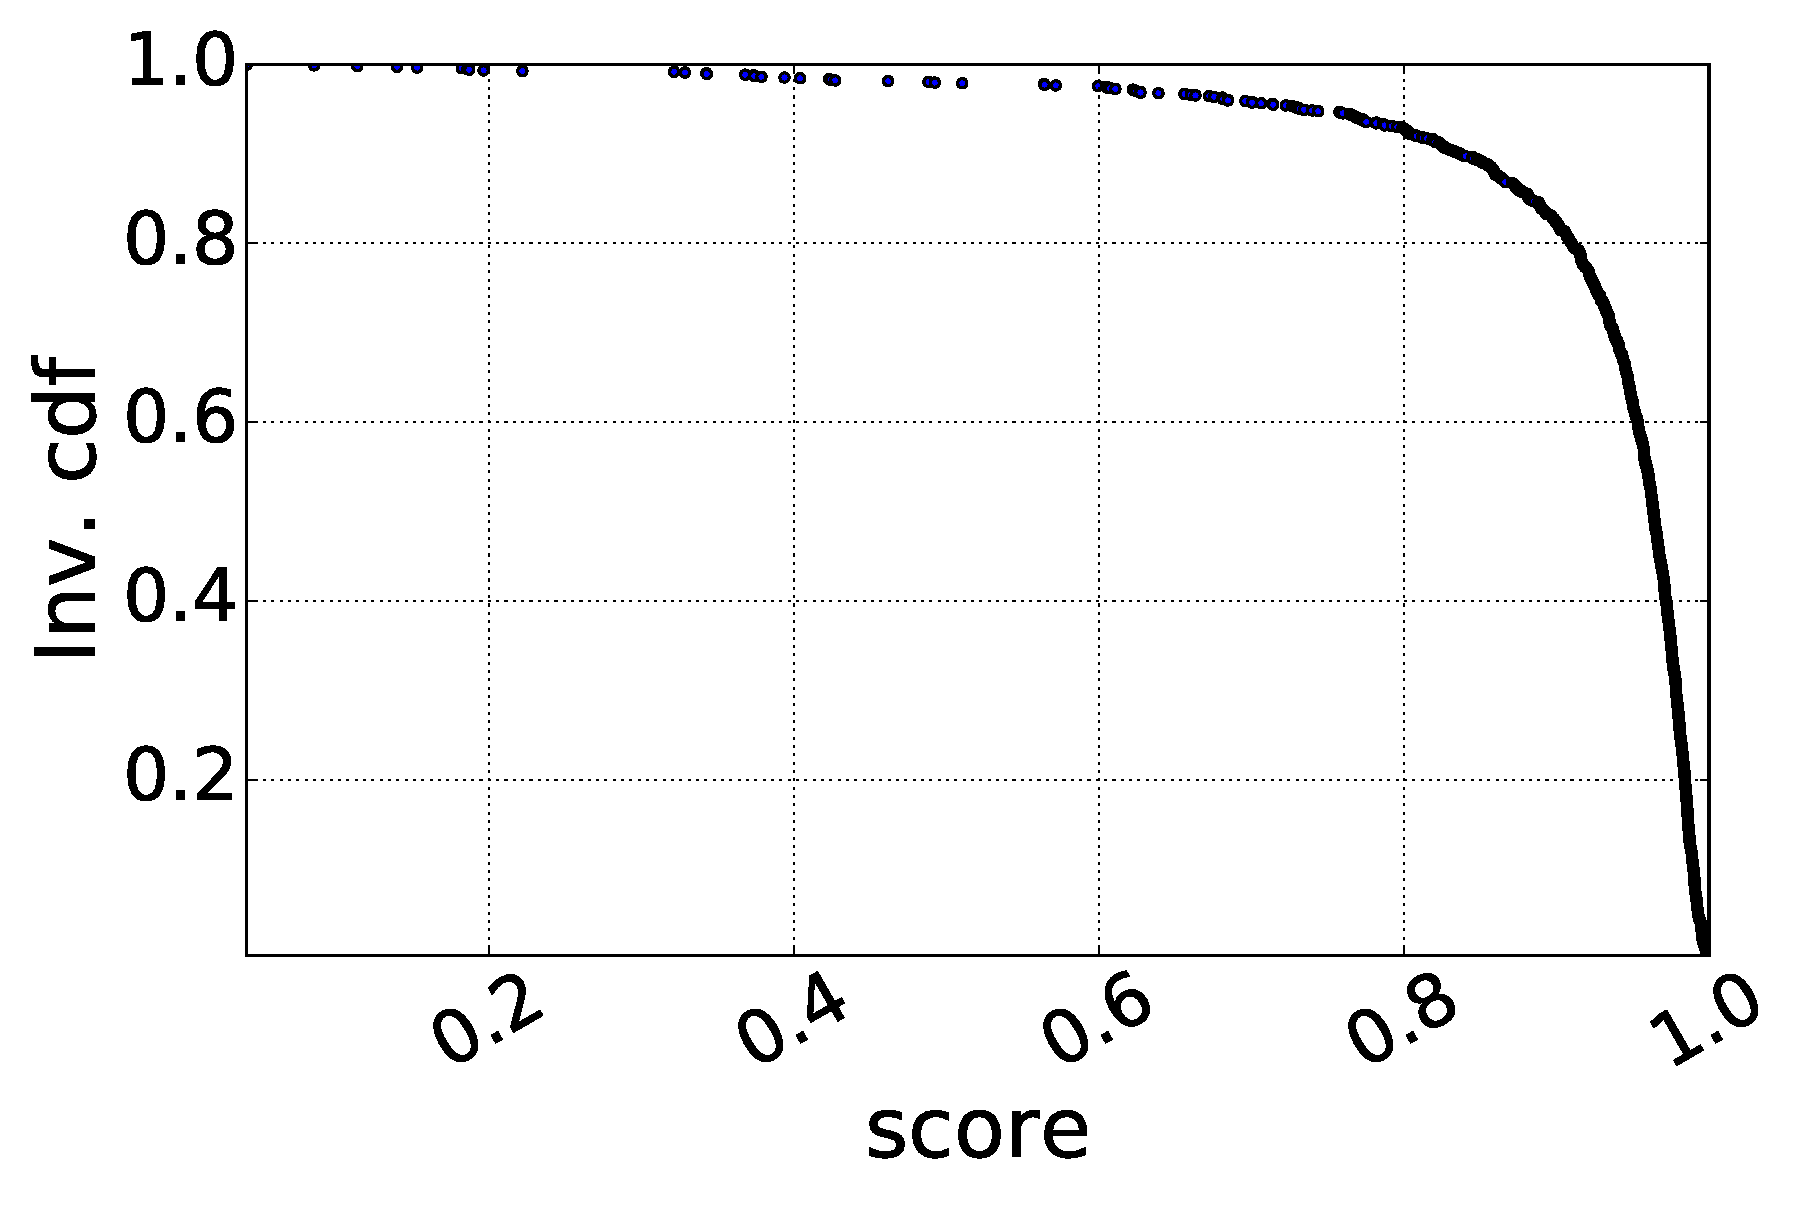
\includegraphics[width=\linewidth]{img/GroupeDense/#1/Percentil/Distribution_percentil_FixTime_top155.eps}
		\caption{Duration: $p_{\delta}$}
	\end{subfigure}
	
	\begin{subfigure}{0.48\linewidth}
		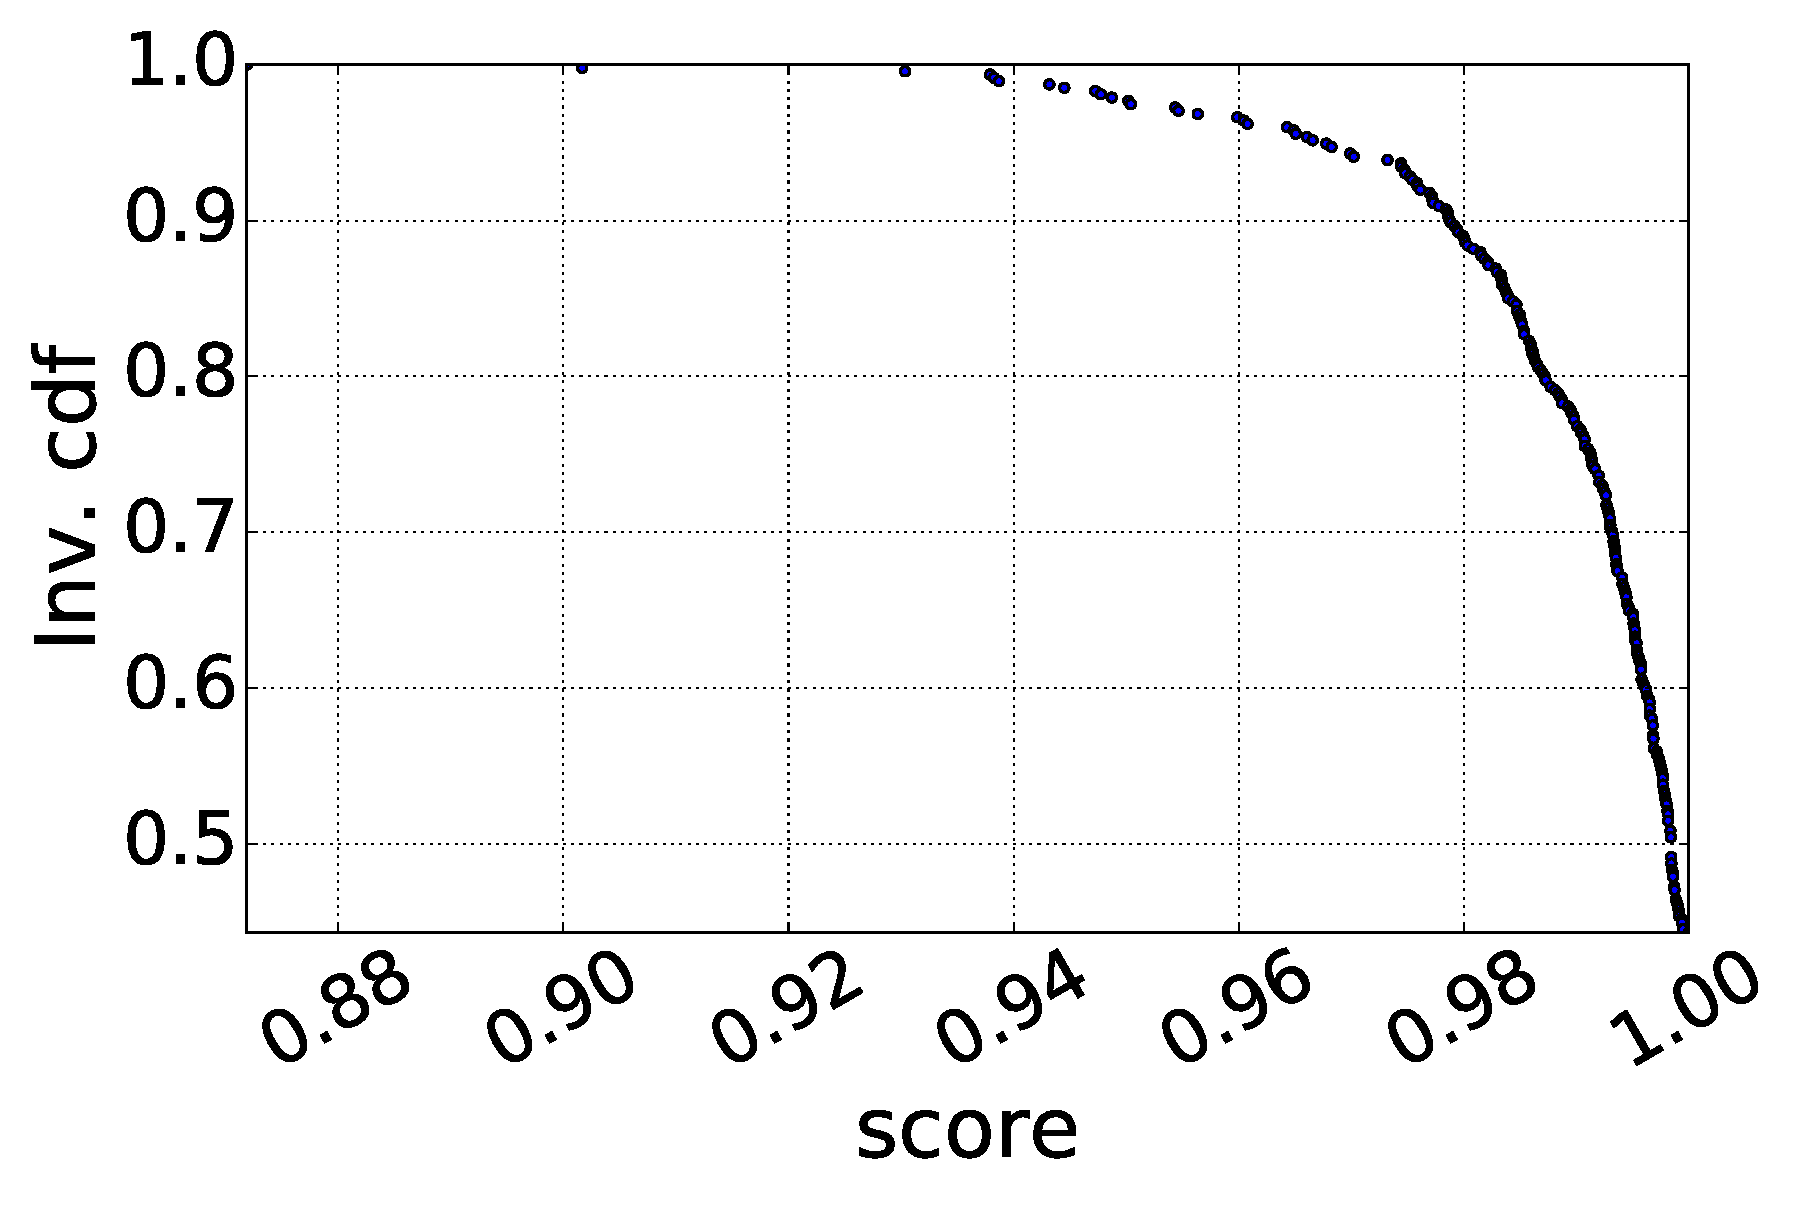
\includegraphics[width=\linewidth]{img/GroupeDense/#1/Percentil/Distribution_percentil_Rand_top155.eps}
		\caption{Node set:$p_{node}$}
	\end{subfigure}\hfill
	\begin{subfigure}{0.48\linewidth}
		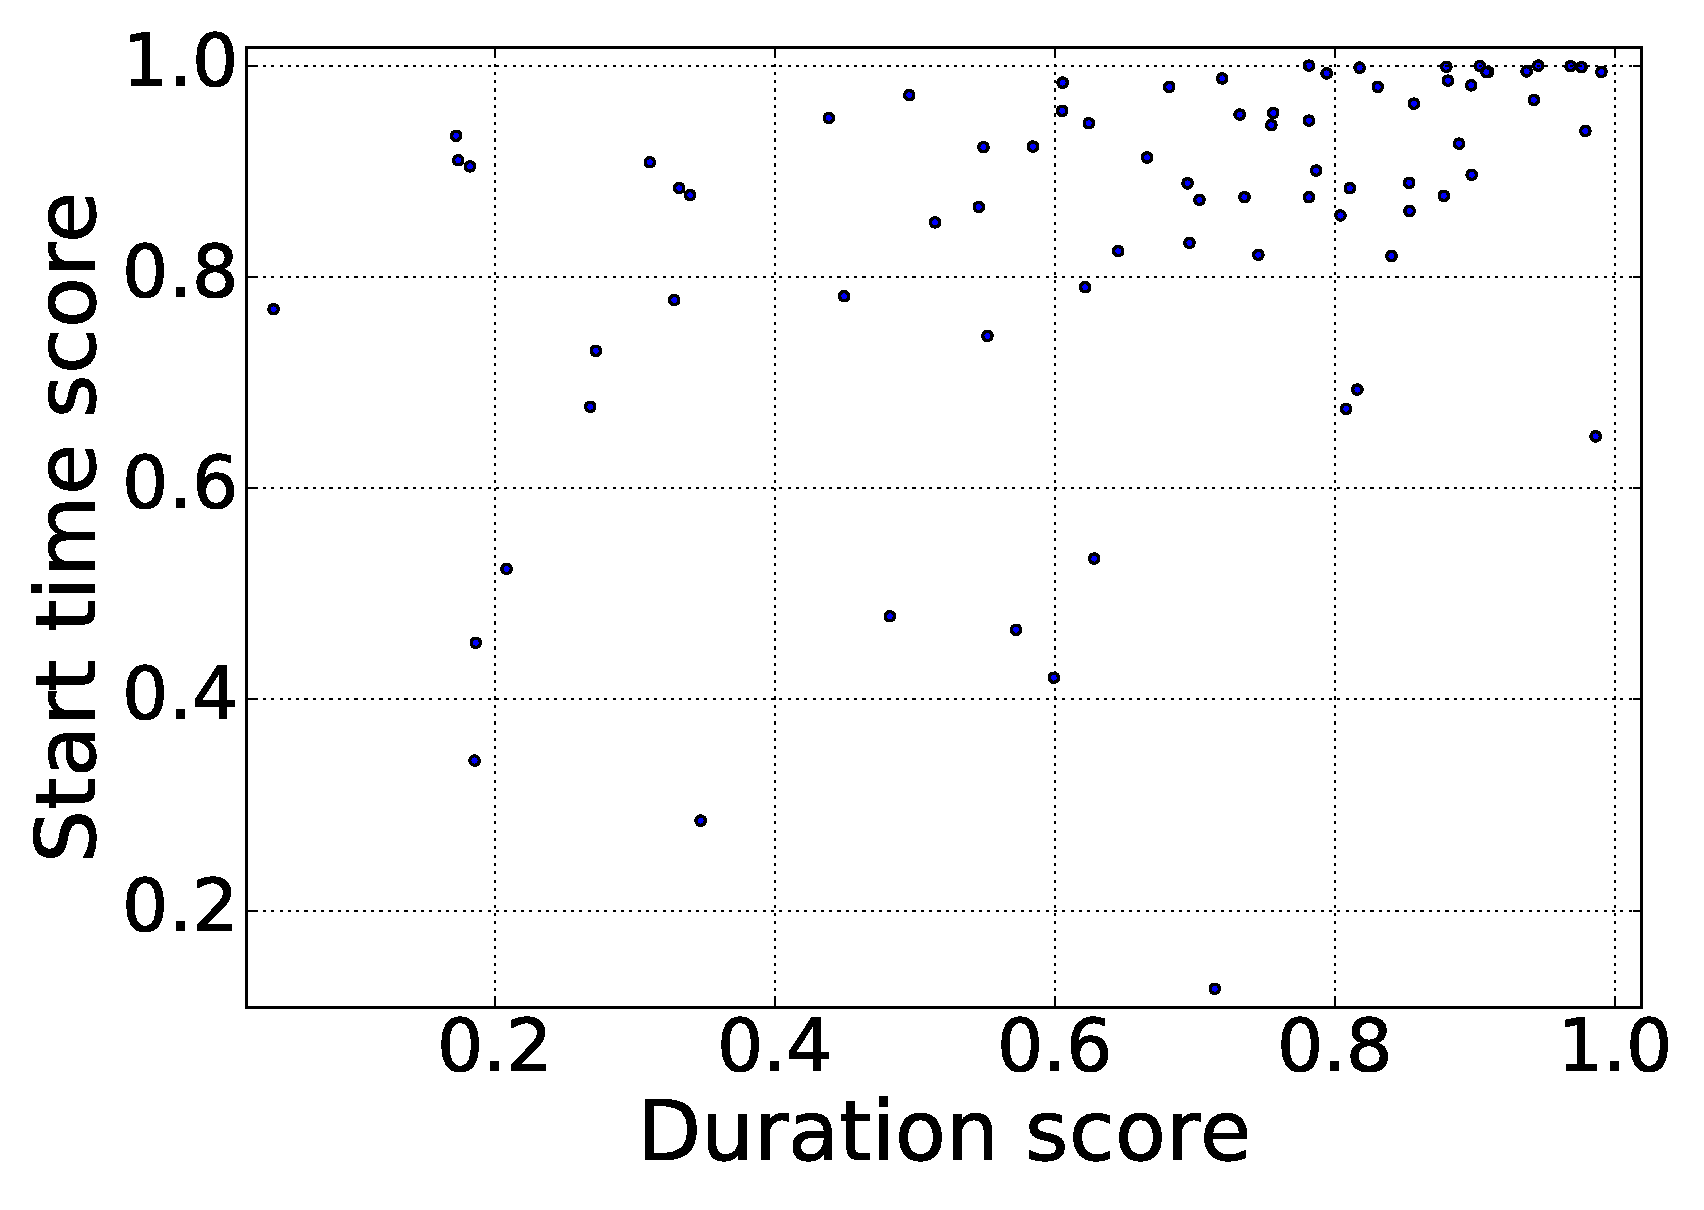
\includegraphics[width=\linewidth]{img/GroupeDense/#1/ecart/relationFixTime_FixDuration.eps}
		\caption{Correlation between start time and duration aspects.}
	\end{subfigure}
	\caption{Inverse cumulative distribution of scores for each aspect for the dataset #2.}
	\label{fig:dit_#3}
	\end{figure}
}
\newcommand{\groupcharacFilter}[3]{
	\begin{figure}[h]
	\centering
	
	\begin{subfigure}{0.45\linewidth}
		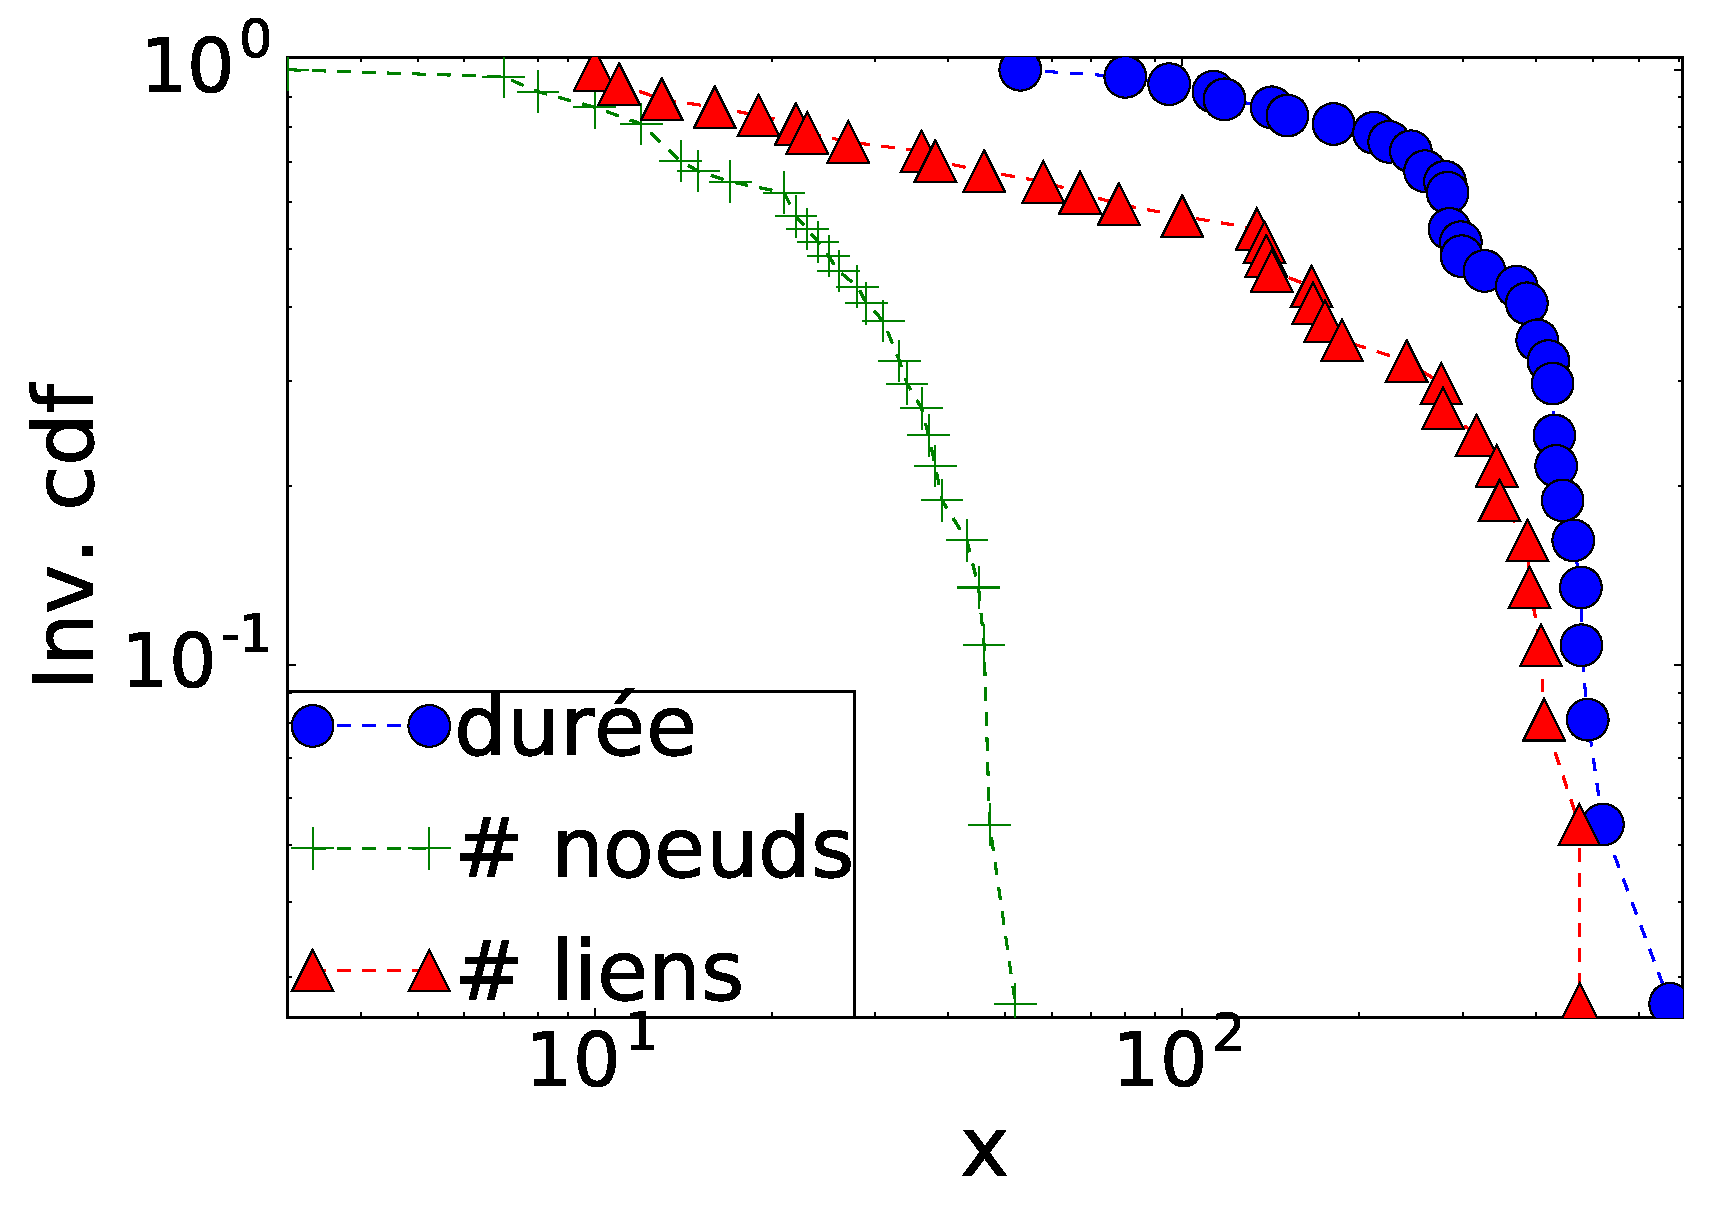
\includegraphics[width=\linewidth]{img/GroupeDense/#1/filter/Distrib_apres_filtre_best}
	\end{subfigure}\hfill
	\begin{subfigure}{0.45\linewidth}
		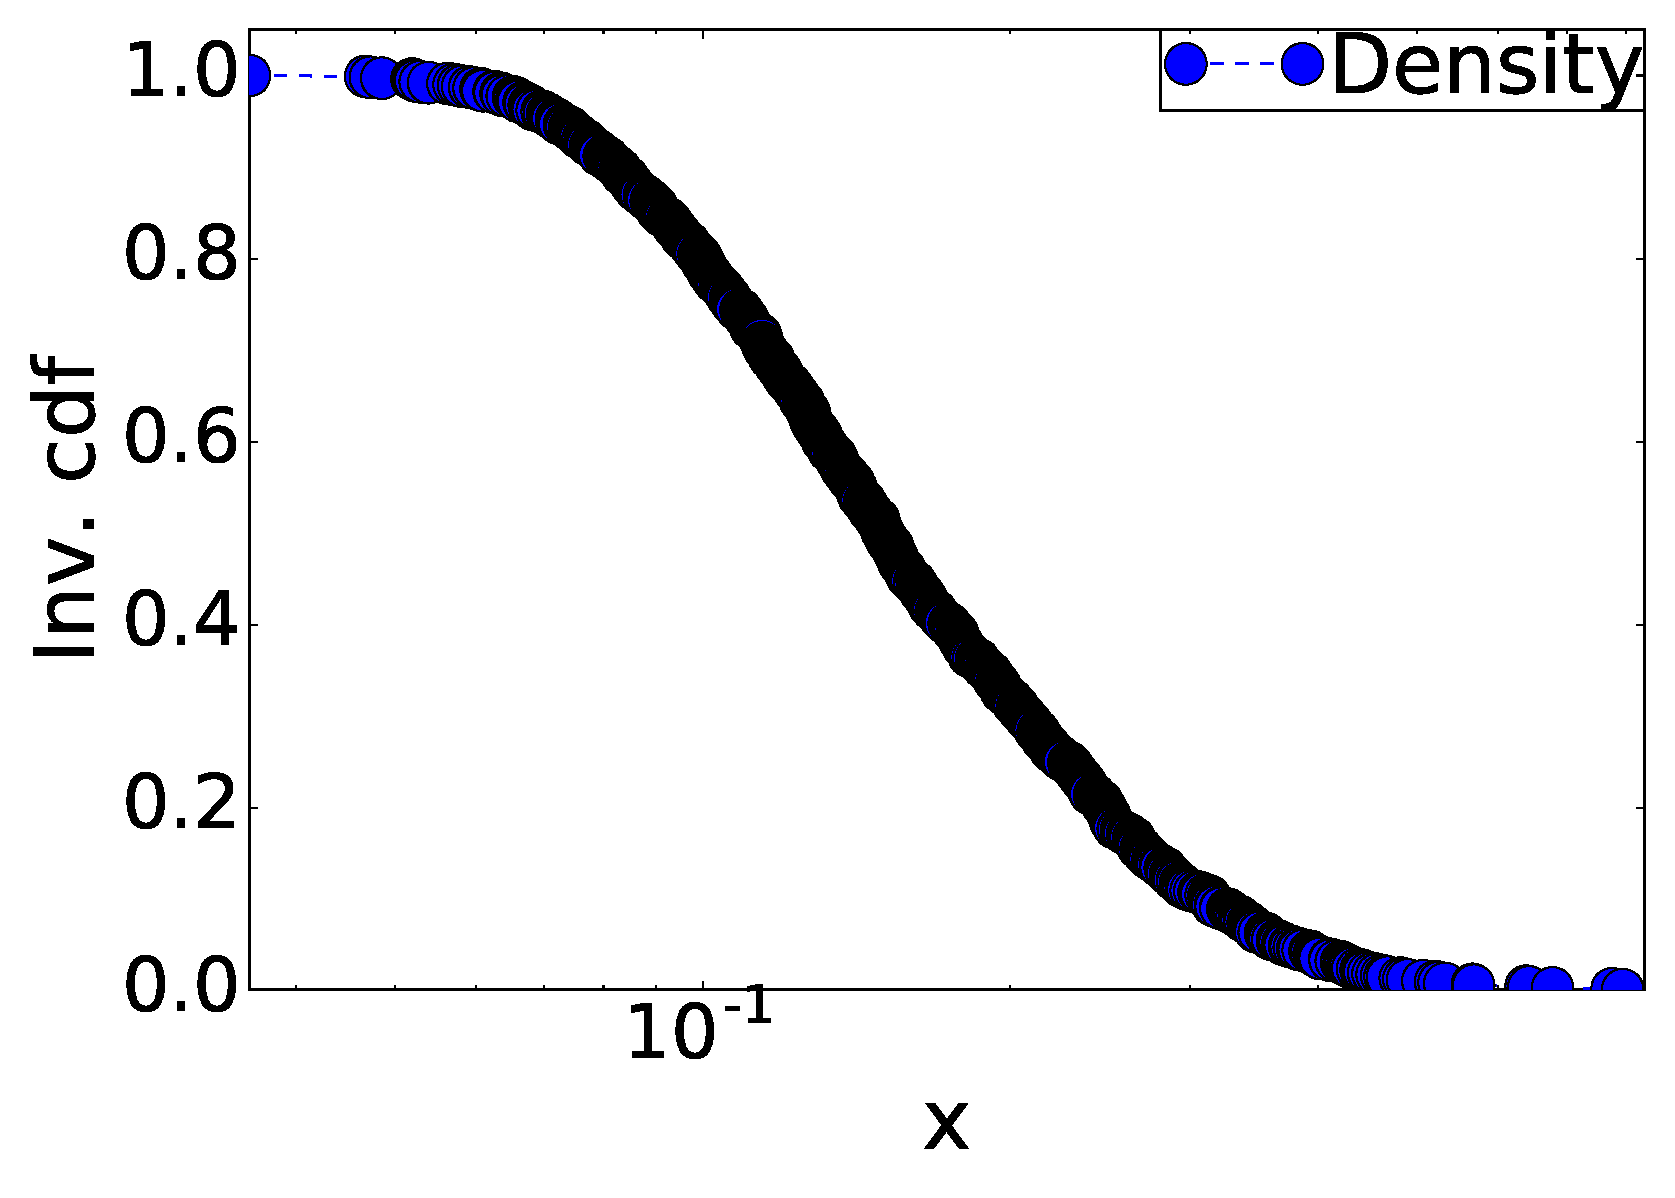
\includegraphics[width=\linewidth]{img/GroupeDense/#1/filter/Distrib_apres_dens.eps}
	\end{subfigure}
	\caption{Inverse cumulative distributions of the number of links, nodes and duration in (a) and density in (b) for the candidates captured by our method on the #2 dataset.}
	\label{fig:distri_group_#3_filter}
	\end{figure}
}

%----------------------------------------------------------------------------------------
%	MARGIN SETTINGS
%----------------------------------------------------------------------------------------

\geometry{
	paper=a4paper, % Change to letterpaper for US letter
	inner=1.5cm, % Inner margin
	outer=2.5cm, % Outer margin
	bindingoffset=1cm, % Binding offset
	top=1.5cm, % Top margin
	bottom=1.5cm, % Bottom margin
	%showframe,% show how the type block is set on the page
}

%----------------------------------------------------------------------------------------
%	THESIS INFORMATION
%----------------------------------------------------------------------------------------
\dominitoc

\thesistitle{Conversations, Groupes et Communautés dans les Flots de Liens} % Your thesis title, this is used in the title and abstract, print it elsewhere with \ttitle
\supervisor{Clémence \textsc{Magnien}\\ Matthieu \textsc{Latapy}} % Your supervisor's name, this is used in the title page, print it elsewhere with \supname
\examiner{..} % Your examiner's name, this is not currently used anywhere in the template, print it elsewhere with \examname
\degree{Doctor of Philosophy} % Your degree name, this is used in the title page and abstract, print it elsewhere with \degreename
\author{Noé \textsc{Gaumont}} % Your name, this is used in the title page and abstract, print it elsewhere with \authorname
\addresses{} % Your address, this is not currently used anywhere in the template, print it elsewhere with \addressname

\subject{... Sciences} % Your subject area, this is not currently used anywhere in the template, print it elsewhere with \subjectname
\keywords{} % Keywords for your thesis, this is not currently used anywhere in the template, print it elsewhere with \keywordnames
\university{\href{http://www.university.com}{University Name}} % Your university's name and URL, this is used in the title page and abstract, print it elsewhere with \univname
\department{\href{http://department.university.com}{Department or School Name}} % Your department's name and URL, this is used in the title page and abstract, print it elsewhere with \deptname
\group{\href{http://researchgroup.university.com}{Research Group Name}} % Your research group's name and URL, this is used in the title page, print it elsewhere with \groupname
\faculty{\href{http://faculty.university.com}{Faculty Name}} % Your faculty's name and URL, this is used in the title page and abstract, print it elsewhere with \facname

\hypersetup{pdftitle=\ttitle} % Set the PDF's title to your title
\hypersetup{pdfauthor=\authorname} % Set the PDF's author to your name
\hypersetup{pdfkeywords=\keywordnames} % Set the PDF's keywords to your keywords

\newcommand{\REF}{\textcolor{red}{REF}}
\newcommand{\com}[1]{\textcolor{red}{#1} }



